% Ubah judul dan label berikut sesuai dengan yang diinginkan.
\section{Tinjauan Pustaka}
\label{sec:tinjauanpustaka}

\begin{enumerate}[label=\Alph*.]
    \item Robot Humanoid
    \label{subsec:robothumanoid}

    \hspace*{1em} Robot humanoid adalah robot yang meniru penampilan keseluruhan manusia dan mampu berinteraksi dengan lingkungan dan peralatan sekitarnya. Secara umum, robot humanoid terdiri dari komponen kepala, badan, dua lengan, dan dua kaki, dengan sendi gerak yang meniru struktur tubuh manusia, yang dikendalikan menggunakan servo.

    \item Sensor Load Cell
    \label{subsec:sensorloadcell}

    \hspace*{1em} Sensor Load Cell adalah sensor yang digunakan untuk mengukur tekanan atau gaya yang diterapkan pada suatu objek. Sensor ini bekerja berdasarkan prinsip perubahan resistansi yang terjadi pada strain gauge yang terpasang pada sensor.

    \begin{figure}[h]
        \centering
        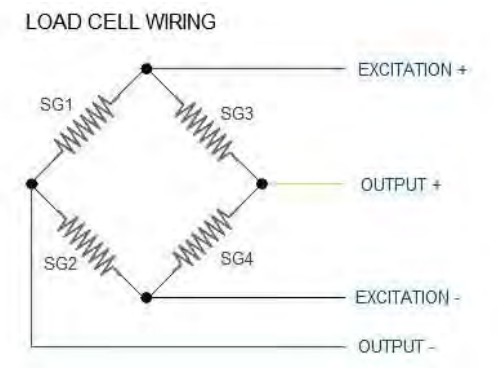
\includegraphics[width=0.35\textwidth]{./gambar/wheatstone_loadcell.png}
        \caption{Rangkaian Wheatstone Bridge pada Load Cell\cite{rahman2018autonomous}.}
        \label{fig:Wheatstone_Bridge}
    \end{figure}
    
    \begin{equation}
      V_{\mathrm{out}} = V_{\mathrm{in}} \cdot \frac{R_2 \cdot R_3 - R_1 \cdot R_4}{(R_1 + R_2) \cdot (R_3 + R_4)}
      \label{eq:Wheatstone_Bridge}
    \end{equation}
    
    \hspace*{1em} Di dalam sensor Load Cell, sistem sudah dilengkapi dengan rangkaian Wheatstone Bridge. Rangkaian Wheatstone, seperti ditunjukkan pada Gambar \ref{fig:Wheatstone_Bridge}, adalah rangkaian yang digunakan untuk mengukur perubahan resistansi yang memiliki sensitivitas tinggi \cite{rahman2018autonomous}. Untuk mengukur perubahan resistansi, digunakan persamaan Wheatstone Bridge seperti pada Persamaan \ref{eq:Wheatstone_Bridge}. 

    \item \textit{Real Time Operating System} (RTOS)
    \label{subsec:rtos}

    \hspace*{1em} Real-Time Operating System (RTOS) adalah komponen penting dalam sistem tertanam modern. Kemampuannya dalam mengelola tugas konkuren secara efektif memungkinkan sistem untuk memproses data dari berbagai sensor, seperti load cell, secara simultan, dan mengendalikan aktuator dengan presisi tinggi \cite{sayyad2023real}. RTOS memungkinkan sistem untuk menjalankan berbagai tugas secara bersamaan, dengan memprioritaskan tugas-tugas yang lebih penting\cite{digikey2021task}. Hal ini memungkinkan robot untuk merespons dengan cepat terhadap perubahan lingkungan, seperti menjaga keseimbangan, dan secara keseluruhan meningkatkan kinerja dan adaptabilitas robotika yang menggunakan sitem tertanam.

    \item Sistem Kontrol PID
    \label{subsec:sistemkontrolpid}

    \hspace*{1em} Penggunaan sistem kontrol PID (Proportional-Integral-Derivative) adalah metode yang umum digunakan dalam kontrol servo motor. Sistem ini membantu menjaga keseimbangan dan stabilitas robot dengan mengoreksi pergerakan berdasarkan nilai error yang dihasilkan dari perbedaan antara posisi aktual dan posisi yang diinginkan. PID terdiri dari tiga komponen utama: kontrol proporsional (P), integral (I), dan diferensial (D). Masing-masing komponen ini berfungsi untuk memperbaiki kesalahan dengan cara yang berbeda.

    \hspace*{1em} Gabungan dari ketiga komponen ini membentuk kontrol PID yang efektif dalam menjaga keseimbangan dan stabilitas robot. Pengaturan parameter $K_p$, $K_i$, dan $K_d$ yang tepat sangat penting untuk memastikan sistem berkinerja optimal dan responsif.

    \begin{equation}
      \mathrm{Koreksi} = K_p \cdot \mathrm{error} + K_i \cdot \int_{0}^{t} \mathrm{error} \cdot dt + K_d \cdot \frac{d\mathrm{error}}{dt}
    \end{equation}

    \item Pusat Tekanan
    \label{subsec:pusattekanan}

    \hspace*{1em} Pusat tekanan adalah titik dimana semua gaya terkonsentrasi pada titik tersebut tanpa ada momen torsi\cite{hawley2016external}. Dalam pusat tekanan ini terdiri dari beberapa tekanan yang kemudian dihitung nilainya berdasarkan luas penampang tersebut hingga didapatkan posisi pusat tekanan tersebut. Pusat Tekanan memiliki hubungan dengan keseimbangan robot terutama pada titik pusat gravitasi\cite{arifin2017implementasi}.

    \begin{equation}
      X_{\mathrm{cop}} = X_0 + \frac{(F2 + F4) \cdot dx}{F1 + F2 + F3 + F4}
      \label{eq:COP_X_1}
    \end{equation}

    \begin{equation}
      Y_{\mathrm{cop}} = Y_0 + \frac{(F1 + F2) \cdot dy}{F1 + F2 + F3 + F4}
      \label{eq:COP_Y_1}
    \end{equation}


    \begin{figure} [h] \centering
      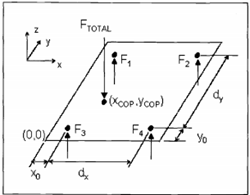
\includegraphics[width=0.3\textwidth]{gambar/Konsep_Letak.png}
      \caption{Konsep Tata Letak Pusat Tekanan\cite{resna2005}.}
      \label{fig:Konsep_Letak}
    \end{figure}

    \hspace*{1em} Gambar \ref{fig:Konsep_Letak} menunjukkan konsep peletakkan sensor tekanan. Dari konsep tersebut dapat dihitung pusat tekanan dengan menggunakanan Persamaan \ref{eq:COP_X_1} dan Persamaan \ref{eq:COP_Y_1}.
\end{enumerate}